\section{Observations}

\subsection{Observations Task 1}
\todo{what information could be retrieved from the implemented technique?}
\todo{was the task accomplished?}
\todo{pros, cons, improvements}

task 1a
- taking some general attributes such as those in $S_{attr}$ mainly show rather obvious relations:
    > \texttt{AANTAL\_INW} == \texttt{AANTAL\_HH}
    > \texttt{OPP\_TOT} inverse \texttt{BEV\_DICHTH}
    > \texttt{STED} inverse \texttt{OAD}
- quite some attributes with a few outliers that mess up the scale of the axis
\texttt{OPP\_TOT}, \texttt{OAD}, \texttt{AANTAL\_INW}, \texttt{AANTAL\_HH}
    this makes it harder to detect relations between the attributes of the more general municipalities, because they lie very close to each other on the axis.

Let us now the questions we posed in the section Tasks,
- answers to questions: \texttt{AANT\_INW} <-> \texttt{BEV\_DICHTH}: Súdwest-Fryslân, Lelystad, Haarlemmermeer, Apeldoorn, Ede, Emmen do not adhere


task 1b
- again because the scaling, it also becomes harder to compare municipalities
\texttt{OPP\_TOT}, \texttt{OAD}, \texttt{AANTAL\_HH},
-> con: outliers rack up the scaling -> solution: scale the axes to selection
- student cities have highest percentage of single households (\texttt{P\_EENP\_HH})
- municipalicites with low \texttt{STED} value fluctuate more on the other attributes

\begin{figure}[h!]
    \centering
    \captionsetup{justification=centering,margin=2cm}
    \begin{subfigure}[t]{0.48\textwidth}
        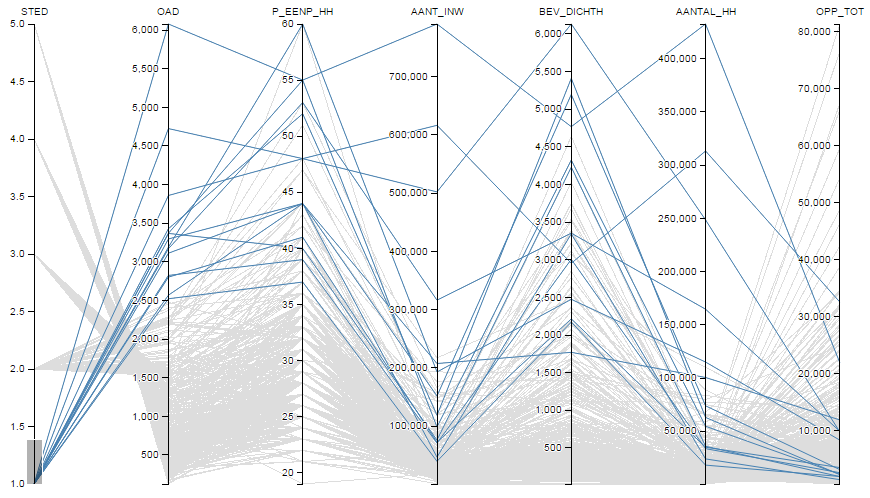
\includegraphics[width=\textwidth]{img/pcp_STED1.png}
        \caption{ }
    \end{subfigure}
    \begin{subfigure}[t]{0.48\textwidth}
        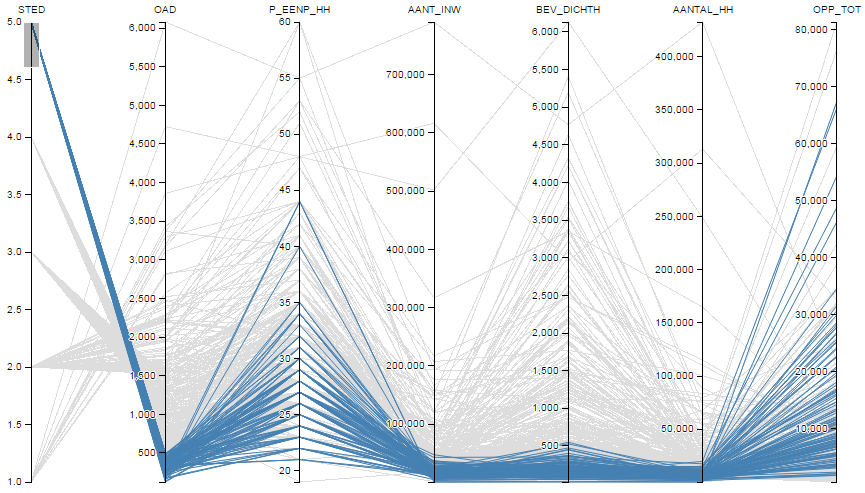
\includegraphics[width=\textwidth]{img/pcp_STED5.png}
        \caption{ }
    \end{subfigure}
    \label{fig:pcp_sted}
    \caption{Parallel Coordinate Plots highlighting the municipalities with a \texttt{STED} value of 1 (a), and a \texttt{STED} value of 5 (b)}
\end{figure}

\subsection{Observations Task 2}
\todo{what information could be retrieved from the implemented technique?}
\todo{was the task accomplished?}
\todo{pros, cons, improvements}

